\documentclass[a4paper, 12pt, oneside]{book}

\usepackage{times}
\usepackage{verbatim}
\usepackage{color}
\usepackage{url}
\usepackage{graphicx}
\usepackage{array}
\usepackage{theorem}
\usepackage{amssymb}
\usepackage{amsmath}
\usepackage{amsfonts}
\usepackage{setspace}
\usepackage{pdfpages}
\usepackage{wallpaper}
%\CenterWallPaper{.4}{watermark.pdf}

% uncomment this if you want to indent the first paragraph
%\usepackage{indentfirst}

% uncomment this if you want to make pdf file with hyperlink
% \usepackage[dvipdf,colorlinks=false,unicode]{hyperref}

% uncomment the following and correct them if you want to set 
% set the pdf properties
%\hypersetup{
%	pdfauthor={Tz-Huan Huang},
%	pdftitle={A Benchmark for Region-of-Interest Detection in Images},
%	pdfsubject={Master Thesis}
%}

\usepackage{ntu}

\setcounter{tocdepth}{2}

\pagestyle{plain}

\begin{document}

% cover page
\maketitle

\includepdf{certification.pdf}

% side page, used for printing on spline.
\makeside

\frontmatter


\begin{CJK}{UTF8}{nkai}
\CJKhorz
\makecertification

% comment one of the following unless you are sure you want to 
% have both english and chinese acknowledgements in your thesis

\doublespacing
\begin{acknowledgementsCH}

\setlength{\baselineskip}{1.5em}
口試結束了!學生生涯也快結束了!

最後一兩個月,起初每天都被壓力壓到喘不過過氣,每天都想著什麼時候能結束?直到最後一個禮拜,我才意識到所剩的時間不多,既然這都是學生生涯的Last Shot了,有什麼理由不讓他變成Best Shot?於是用力的提起勁來做事。想著要給老師驚喜,也想著不要讓老師失望,也不想讓自己後悔。很高興最後我沒有留下遺憾。最重要的是我覺得沒有愧對老師,也沒有愧對自己!

一路走來,真的很感謝老爸以及家人的支持。感謝小ㄅㄟˊ在所有事情上面的體諒,妳的體貼是支持我最大的動力。感謝一路走來的戰友們楊證諺、大黃、小黃、阿崴、明鑫、土涵、田波、阿璽、痞子,無論是歡笑出遊或是痛苦熬夜,都很榮幸能跟你們一起度過。感謝特地捎來祝褔的摳拉、鳥鳥、大喬,你們的祝福讓我多一分勇氣站在台上。很感謝陪我一起在第一戰線被老師念、又陪我在最後戰線在R544待到天亮的小捲。感謝葉老大這位兩年來數不清次數在關鍵時刻給我幫助的靠山。很感謝大黃還有學弟妹Larry、Jean Wang、何佳儒口試時辛苦幫忙食物飲料!很感謝鐵哥,每次跟你聊真的都學到很多。感謝許碩傑、黃鈞愷,你們永遠是我最敬愛的學長。最感謝的是老師、每次Meeting都給我不同的啟發、困惑的時候都給我明確的方向,還有感謝老師對我的信任,非常感謝老師當初願意指導我,我真的覺得很幸運,謝謝老師!

最後寫給還沒口試的好朋友們,如果你們看到這篇文,不要生氣覺得我那麼快就開始寫畢業感言,而是看到前面說的:「最後三四天,才驚覺時間不多」。當研究生,難的就是要相信,相信自己走在對的路上,相信自己正在做對的事情,看不到終點的比賽最難完成,如果你自己都不能相信現在正在做的是對的事情,那短短的"printf();"都可以敲一分鐘。請不要懷疑自己,當你「相信」自己能畢業,下一階的問題就是,我要以什麼姿態畢業,我要畢業的得過且過還是讓自己驕傲?當問題從被動變成主動,寫Code也會從被動變成主動!你們個個都比我強不只一點點,我都把你們當神在拜了,要相信自己呀!加油!



\end{acknowledgementsCH}

\begin{abstractCH}

\setlength{\baselineskip}{1.5em}
在本篇論文中,我們對於以深度影像為基礎達成即時頭部軌跡追蹤之問題提出了兩種不同的方法。在方法一中,我們在深度圖上對使用者的正臉取樣產生點雲(Point Cloud),並使用這些點雲以最小平方法計算出最佳近似的平面,再將臉部輪廓以最小平方法計算出最佳近似的橢圓,以此平面之法向量及橢圓之傾斜角計算出頭部之旋轉角度。在方法二中,我們使用梯度坡降法迭代地將特定距離函數進行最佳化,此方法可算出更精準的旋轉角度及移動距離。我們所提出的這兩個方法,在單一CPU運算下皆可達到30fps的計算速度。在此系統所使用之攝影器材─Microsoft Kinect以及Asus Xtion Pro,乃較為普及、平價、易取得且易使用的深度攝影機,其優點亦伴隨著較高的拍攝雜訊。為了使系統得以不被環境光線改變所影響,我們只利用其拍攝出之深度影像為輸入來源做計算。在本篇論文中,我們證明,三維空間中,六個自由度的即時頭部軌跡追蹤,是可以經由分析帶有雜訊之深度影像達成的。

 

\noindent\bf{關鍵字: 即時頭部運動軌跡追蹤; 深度影像; 三維樣板比對; 迭代最佳化; 最小平方法}
\end{abstractCH}

\begin{abstractEN}
In this thesis, we propose a system to estimate head poses only using depth information in real-time. Two methods are developed. First, assuming that a head can be approximated by a bounding box, we find the best fitted plane for the frontal face by the least square error method. Thus, the normal vector of this plane represents the head orientation. Second, an optimization method based on 3D model fitting is developed. We iteratively minimize the distance between source and target point clouds of a user's head. This method is more robust and the results are more precise. Both of the proposed methods give fully real-time responses (30fps) without needing the GPU speedup. We adopt a commodity depth sensor named Microsoft Kinect as well as Asus Xtion, and use the depth image as the only input so that our system will not be affected by illumination variations. The simplicity of this acquisition device comes at the cost of frequent noises in the acquired data. We demonstrate that 6 degree of freedom real-time head motion tracking in 3D space can be achieved with noisy depth data.

 

\noindent\bf{Keywords: Real-Time Head Motion Tracking; Depth Image; Kinect; 3D Template Matching; Iterative Optimization; Least Square Method}

\end{abstractEN}

\begin{comment}

%\category{I2.10}{Computing Methodologies}{Artificial Intelligence --Vision and Scene Understanding} \category{H5.3}{InformationSystems}{Information Interfaces and Presentation (HCI) -- Web-based Interaction.}

%\terms{Design, Human factors, Performance.}

\keywords{Head Pose Estimation \and Depth Map \and Kinect \and Least Square Error Plane \and Optimization \and Gradient Decent Algorithm \and Nose Tracking}

\end{comment}

\tableofcontents
\end{CJK}
\doublespacing
\listoffigures
%\listoftables

\mainmatter
\spacing{2.5}
% input your thesis here
\chapter{Introduction}
\label{c:intro}
In recent years, the way that humans have their interaction with computers has become a well concerned issue. It turns out that people tend to be more attracted by the so called ``Natural User Interface(NUI)''. A natural user interface allows the user interacts with the computer through intuitive actions related to natural, everyday human behavior. Instead of using the old fashioned tools such as keyboards, mouses, or joysticks, which are the combination of several buttons and sensors, people would rather like making natural moves and intuitive body languages. In this way, the interaction between human and computer becomes more similar to the interaction between human and human. Moreover, it will be much easier for people to learn how to use the computer. For example, A ``nod'' may indicates ``yes'' and a ``head shake'' may indicates ``no'', and these natural moves will be able to take the place of clicks on the mouse or taps on the keyboard.

There are plenty of topics to be discussed within this area. For instance, body languages, gestures recognition, speech recognition, head pose estimation, etc. In this thesis, we focus on the area of head motion tracking. The main motivation is that human head motion information is important for computers to understand the messages or commands that users want to deliver. In other words, head motion information is an key element to the analysis of human behavior. The  results of such analyses will have a wide range of usage.

For example, an safety monitoring system installed in a car can alarm as a warning to the driver when he loses his concentration. In an virtual reality system, a head mounted display needs to know the user's head motion information before it can decide what content should be displayed to the user. 

Besides, with the fast growing of computer animation industry, the value of head motion information increases. An obvious reason is that it takes enormous time for artists to make the virtual characters perform even the simplest move. In order to make the characters move as realistically as possible, animators manually set several key frames for each single move, then they manually set the interpolation curve between each key frames. Note that every step within this task takes huge amount of time. However, with the help of head motion information, animators will be able to make the virtual characters move and turn their heads as a live imitation of the real human performer, but just spend much shorter period of time. 

Moreover, when it comes to the most popular video game consoles, say Nintendo Wii, Microsoft XBox 360 or Sony PlayStation, we would like to know the reason why they are so successful, how did they succeed. The answer is: The key to success lies on the type of controller. The Wii remote wireless controller was a brand new type of controller among all of the video game consoles. Thus, Nintendo Wii had had defeated any other competitors at that time and stood out as a milestone in the console game's history. Before long, Sony and Microsoft both released their new devices in order to compete with Nintendo Wii. Sony promoted PlayStation Move while Microsoft promoted Xbox Kinect. PlayStation Move is a handheld remote controller similar to Wii Remote that is capable of capturing 3D motion of players' both hands, while Kinect is a camera alike device which is able to help capturing the 3D motion of players' whole body skeletons without requiring players to wear or hold and controllers. All of these technologies has brought nowadays console games and the user experiences to a whole new generation. However, none of them is capable of tracking the plays' head motions. Undoubtedly, head motion information should be include into natural user interface together with gestures as well as spoken commands.

All of the mentioned examples point to the same conclusion that head motion information is important and we should make use of it.
% talk about ROI, what it is, why it is important
\section{Issues in Head Motion Tracking}
There are several difficulties within this head motion tracking task. Different systems may encounter different difficulties because of the different approaches they depend on and the different purposes they are up to. These issues may or may not all appear. 
\begin{enumerate}
\item Real-time Response: Speed versus precision, is always a tradeoff in most of computer science works. Head motion tracking is one of them. If we like to do real-time computation, we should simplify the comparing method as much as we can, stop the iteration as early as we can. However, we won't be able to do more detailed analysis and thus produce a less accurate tracking result. In an interactive system such as video game or video communication, the response time directly decides how the user feels. Even a small time delay may not be tolerable in these conditions. A small range of inaccuracy, however, is acceptable. In this kind of systems, real-time constraint is of top concern.
\item Variable Illumination: Most image based methods assume fixed lighting, so that every point of the object can be considered to have fixed color intensity. However, even with well-controlled lighting, intensity of an object still changes as it moves, let alone the fact that the environment of a practical system seldom matches the ``fixed lighting'' assumption. On the other hand, systems depending on marker or depth sensor may not encounter this issue.
\item Visibility: Feature points may disappear due to occlusion when the user rotates his head. When the feature points are gone, feature points correspondence analysis fails, then the motion estimation will be forced stop. As a consequence, feature-based methods often have rotation angles limitations owing to the visibility issue.
\item Rigid Head Constraint: Most head motion tracking methods assume a rigid human head to be observed. A rigid human head indicates that there is no relative motion between any points on the head, so that one can further assume that the geometrical relation between each feature points are fixed. However, because of the facial expressions, the blinks, the waving hair, or the talking mouth, human heads are usually non-rigid, thus the difficulty of this task is increased.
\end{enumerate}

%\section{Contribution}
%The main contribution of this works are...

\section{Organization}
The rest of this thesis is organized as follows. A brief introduction to several great related works to this topic is written in Chapter \ref{c:related}. We divide the previous works into several categories for further discussion, then we compare out work to state-of-the-art methods and propose our contributions. Chapter \ref{c:overview} is the overview of our system. The hardware introduction and system architecture are described in this chapter. The two proposed approaches for head motion tracking are then illustrated in Chapter \ref{c:method}. This chapter specifies work flows and implementations of both approaches in detail. Some procedures, which are identical in both of the two approaches, are introduced first. Then we elaborate on the unique procedures of both approaches, respectively. Results of the proposed 3D head pose estimation are demonstrated in Chapter \ref{c:result}. We conclude this thesis in Chapter \ref{c:conclusion}, and future works are discussed.
\chapter{Related Works}
\label{c:related}

% talk about ROI, what it is, why it is important
Previous researches about head motion tracking can be divided into several categories depending on the type of data required (i.e., 2D image or depth map). A comprehensive survey on methods based on 2D images is given by \cite{Murphy:09:SURVEY}. We can further divide the 2D image-based algorithms into two types, feature-based \cite{Yang:02:MBHPTWS,Vatahska:07:FBHPEFI,Matsumoto:00:AAFRTSVIOHPAGDM,Yao:04:EMBLHMRFM,Whitehill:08:ADATFBFHPT} and appearance-based \cite{Morency:03:PEU3VBE,Balasubramanian:07:BMEAFFPIHPE,Osadchy:07:SFDPEEBM,Storer:09:3DMAM,Chen:03:HPEUFML,Whitehill:08:ADATFBFHPT} methods. Feature-based methods focus on the specific facial feature points while appearance-based methods look at the entire face.

\section{Feature-Based Methods}
Feature-based methods tend to find feasible matches either between object features and image features or between features of consecutive video frames. Yang et al. \cite{Yang:99:USP} estimate the head pose by first tracking three facial feature points, which are the eyes and the nose tip, and then using gradient decent algorithm to optimize the defined distance function modeled by rotation and translation parameters. The approach of \cite{Yang:02:MBHPTWS} acquires input video from vertical stereo cameras so that they can easily remove outliers through epipolar system in the feature matching step. Although this approach achieves real-time performance, a personal face model and some user hints are required for initialization. Vatahska et al. \cite{Vatahska:07:FBHPEFI} construct a feature detector using Adaboost in combination with Haar-like features. Then they use a neural network to estimate the three rotation angles of the head pose.

\section{Appearance-Based Methods}
Appearance-based methods use example images of the objects to train a classifier and perform recognition. In head pose estimation, these methods learn a separate detector for each pose, e.g., \cite{Morency:03:PEU3VBE}. Osadchy et al. \cite{Osadchy:07:SFDPEEBM} use a convolutional network to detect the face and its orientation in real-time. Balasubramanian et al. \cite{Balasubramanian:07:BMEAFFPIHPE} and Chen et al. \cite{Chen:03:HPEUFML} both regard this issue as a dimensionality reduction problem, e.g., Construct the mapping from high-dimensional space of facial images to low-dimensional manifold where the data points of head poses lie on. M. Storer et al.\cite{Storer:09:3DMAM} build a 3D morphable appearance model based on registered laser scans of human heads, which is used for fitting the observed data iteratively in an analysis-by-synthesis approach. Generally speaking, appearance-based methods usually have higher computational complexity, and they often extra training steps for each user.

\section{Depth-Based Methods}
On the the other hand, methods relying solely on 2D images share several limitations, the most important of which is that they are so sensitive to illumination variations that they can no longer be robust under weak or no light environment. With the development of fast depth map generating systems such as \cite{Weise:07:F3SWAMC}, many works are inspired to use depth data as additional information to improve color-image based algorithms \cite{Yang:02:MBHPTWS,Morency:03:PEU3VBE,Seemann:04:HPEUSVFHRI}, and several recent works use depth data as their primary information \cite{Breitenstein:08:RTFPEFSRI,Malassiotis:05:RRHPEFRD,Fanelli:11:RTHPEWRRF,fanelli_DAGM11,Weise:11:RPBFA}. Breitenstein et al. \cite{Breitenstein:08:RTFPEFSRI} developed a real time head pose estimation system that is capable of handling large angle rotations of $\pm 90^{\circ}$ yaw, $\pm 45^{\circ}$ pitch and $\pm 30^{\circ}$roll. The method generates many nose candidates. Each candidate  stands for a head pose hypothesis. The reference range images of different poses are rendered offline in the pre-processing stop. By resorting to the parallel computation power of the GPU, they can save these reference images on the graphic card and simultaneously compare the input images to all of them, and finally choose the pose minimizing a predefined cost function. Fanelli et al. \cite{Fanelli:11:RTHPEWRRF,fanelli_DAGM11} formulate pose estimation as a regression problem. They propose to use random regression forests to handle the task for reason that the method has high generalization power and low computational cost. Their system responses in real-time and their results are generally either comparable or superior to that of \cite{Breitenstein:08:RTFPEFSRI}. Weise et al. \cite{Weise:11:RPBFA} estimate facial expression as well as head movement simultaneously. They construct user specific PCA morphable models using iterative closest point (ICP) algorithm first in offline preprocessing. Once more, ICP is used with point-plane constraints for head pose tracking, followed by a maximum a posterior (MAP) estimation for facial expression estimating. Noted that both ICP and MAP estimation have high computational complexity, the authors show that the system can still achieve real-time responses. However, the powerful performance of the system comes at the cost of relatively longer training and preprocessing time for every novice user.

\section{Comparison with the Porposed Method}
Comparing to the above works, the approach that we proposed holds several advantages: Instead of using traditional 2D camera for data acquisition, e.g.\cite{Murphy:09:SURVEY}, both of the proposed approaches purely rely on depth camera so that the systems are not affected by varying lighting conditions. Besides, one of the proposed method has a significantly lower computational cost so that it can achieve real-time performance even on devices that are not equipped with GPUs. As a consequence, this approach will not be limited to powerful devices. Moreover, the capability on enhanced roll angle estimation of our approach outperforms that of the state-of-the-art approach\cite{Fanelli:11:RTHPEWRRF,fanelli_DAGM11} which adopts the same input device as ours.



\newenvironment{definition}[1][Definition]{\begin{trivlist}
\item[\hskip \labelsep {\bfseries #1}]}{\end{trivlist}}

\chapter{Overview}
\label{c:overview}
An overview of the proposed 3D head motion tracking system is illustrated in this chapter. In Section \ref{s:problem}, we give a clear definition for our head motion tracking task. After that, the introduction of the hardware is illustrated in Section \ref{s:hardware}. We will discuss the pros and cons of the hardware, and specify the output format of this device so that the input data of the proposed system can be clear. Section \ref{s:architecture} shows the software system architecture of this system. A high level introduction of the work flow is specified here before going into the implementation details of this work which is specified in Chapter \ref{c:method}. We show our results in Chapter \ref{c:result}. Conclusion and future work are discussed in Chapter \ref{c:conclusion}.

\section{Problem Formulation}
\label{s:problem}
The goal of 3d head motion tracking is to recover the transformation of a person's head in 3D space. The transformation includes rotations with respect to and translations along the three axes. For clear, we give it a definition as the following:
\begin{definition}
The 3D head motion tracking task is the real-time recovery of the six degree of freedom head pose vector of the target head in 3D space given a stream of live performed depth maps.
\end{definition}
In the definition, the head pose vector is a 6$\times$1 vector $v = (r_{x},r_{y},r_{z},t_{x},t_{y},t_{z})^{T}$, which is consisted of six parameters, three of them are the rotation parameters $(r_{x},r_{y},r_{z})^{T}$ and rest of them are the translation parameters $(t_{x},t_{y},t_{z})^{T}$ of the target head in a 3D space.
\begin{figure}
\centering
\includegraphics[width=0.5\linewidth]{./figure/yawpitchroll.pdf}
\caption{Illustration of the three degrees of freedom rotation. Pitch, yaw, and roll are the rotating angle of three mutual orthogonal directions.}
\label{f:rollpitchyaw}
\end{figure}

Figure \ref{f:rollpitchyaw} illustrates the rotation parameters where $r_{x}$ indicates the angle that the head rotates around the $x$-axis, $r_{y}$ indicates the angle that the head rotates around the $y$-axis and $r_{z}$ indicates the angle that the head rotates around the $z$-axis. Borrowing aviation terminology, these rotations are commonly referred to as pitch, yaw, and roll. Pitch angle equals to $r_{x}$; Yaw angle equals to $r_{y}$; Roll angle equals to $r_{z}$. As a more life style description, pitch indicates the motion that the user nods his head, yaw indicates the motion that the user shakes his head left or right, roll indicates the motion that the user tilts his head.

 
\section{Hardware}
\label{s:hardware}
In this thesis, we adopt a depth sensor as our system's input device. Noted that a depth camera is also known as a range camera, and depth data is also known as range data. Instead of those high level depth sensors such as \emph{SwissRanger SR4000}  by \emph{Messa Imaging} which was priced at \$9000 USD or \emph{CamCube} by \emph{PMD Technologies} which was priced at \$12000, we choose the consumer affordable depth cameras such as \emph{XBox Kinect} by \emph{Microsoft} or \emph{Xtion Pro} by \emph{ASUS}, both of them were priced at about \$150 USD.
Xbox Kinect is a motion sensing input device designed for XBox 360 video game console. It was promoted by Microsoft on November, 2010. Kinect is able to capture a color image and its corresponding depth map simultaneously at 30 frames per second, both with a display resolution of 640$\times$480. A similar device named Xtion Pro Live is also released in the same time by ASUS. Figure \ref{f:kinect} shows the devices and the data captured by them, the upper row is Kinect while the lower row is Xtion Pro Live.
\begin{figure}
\centering
\includegraphics[width=1.0\linewidth]{./figure/kinect.png}
\caption{The color image and the corresponding depth map captured by Kinect and Xtion Pro Live, both with resolution of 640$\times$480 at 30 fps.}
\label{f:kinect}
\end{figure}

The sensors with which Kinect equipped including an infrared ray emitter, a visible light camera, an infrared ray receiver, a microphone array and a pedestal motor. While many advanced depth cameras use \emph{``time-of-flight(ToF)''} technique to calculate the distance from the camera to an object by measuring the time it takes for a beam of light to travel to and reflect back from the object's surface, Kinect uses a totally different technique called \emph{``light coding''}. The emitter emits infrared ray which pass through a filter and is scattered into a fixed pattern of speckles. These speckles are then projected onto the scene, see Figure \ref{f:irspeckles}.
\begin{figure}
\centering
\includegraphics[width=0.5\linewidth]{./figure/irspeckles.jpg}
\caption{The projected infrared ray speckles, captured by SONY F717.}
\label{f:irspeckles}
\end{figure}
The reflected pattern, which reveals the distribution of the speckles thus contains the geometrical information of the scene, is then captured by the IR receiver. After decoding the reflected IR pattern, the distance between the camera and the surfaces of object in the scene can be determined, and the corresponding depth map is available.

In brief, Kinect is a non-intrusive, commercially available and consumer affordable device of which the deployment is as easy as an ordinary camera. Furthermore, the user is not required to wear any sensors or markers on his body. The quality of the acquired depth map is not affected by illumination variations.

However, the advantages of this acquisition device come at the cost of high level noises in the acquired data. There is a flicker problem within the acquired depth maps. It is caused by the combination of depth value fluctuation and depth value loss. Our experiments show that the range of fluctuation is about 0.5\% of the distance from the obserced object to the camera in average. That is to say, the error range of every pixel on the depth map is within 0.5cm when the user stands 100cm away from Kinect. Besides, when the IR rays are blocked from being received by Kinect, or there's actually no IR rays reflected from the object surfaces, the depth value of the corresponding pixel on the depth map would be lost. These are caused by specular reflections, transparent materials the horizontal disparity between the IR emitter and the IR receiver, and occlusions. As a consequence, we should handle these issues carefully.

\section{System Architecture}

\begin{figure}
\centering
\includegraphics[width=1.0\linewidth]{./figure/visualflowchart.pdf}
\caption{Visualized work flow of our system. The depth sensor captures the user's actions in real-time, a stream of depth maps is created and is the input of our system. Two methods, least square error method and iterative optimization method, are then applied to do the head motion tracking. The estimated motion vectors are then used to animate virtual avatars at last.}
\label{f:visualized flow chart}
\end{figure}

A high level work flow visualization of our system is illustrated in Figure \ref{f:visualized flow chart}. The depth sensor captures the user's head motion performance in real-time. A stream of depth maps is then created and passed into our system as input data. The third block is the main part of the proposed approach of head pose estimation. Two methods are proposed independently, least square error method and iterative optimization method. Both of them are able to complete the work along. This part which will be discussed in detail in Chapter \ref{c:method}. The fourth block shows that we can retarget the estimated head poses to virtual characters.


\begin{figure}
\centering
\includegraphics[width=1.0\linewidth]{./figure/m1FlowChart.pdf}
\caption{Detailed flow chart of the first proposed motion tracking algorithm which applies least square error method to accomplish the goal.}
\label{f:m1 flow chart}
\end{figure}

Figure \ref{f:m1 flow chart} shows a more detailed flow chart about the first proposed method. This method starts with depth map acquisition for each frame followed by a nose detecting/tracking process. Then we separately accomplish the roll, yaw, pitch angels estimation by two stages: One is to solve a least square error plane approximating to the frontal face for the yaw and pitch angels; The other one is to solve a least square error ellipse approximating to the head's contour for the roll angel. As a result, the nose position shows the former three degree of freedom of the motion vector while the least square methods tells the rest three. The 6-DoF motion vector is then solved. However, the resulting animation driven by these frame by frame motion vectors still has a serious trembling issue. This is mainly because of the low quality of the input depth map. We apply a dynamic weighted averaging filter references from \cite{Weise:11:RPBFA} to tackle this issue. The output of the filter is the final result of this method. This approach performs well in response time which is 30 fps. This makes the system able to give users good experiences. However, when it comes to the precision, the exact number of the rotation angles comparing with the ground truth, it will not show good statistical results.

\begin{figure}
\centering
\includegraphics[width=1.0\linewidth]{./figure/m2FlowChart.pdf}
\caption{Detailed flow chart of the second proposed motion tracking algorithm which applies iterative optimization method to accomplish the goal.}
\label{f:m2 flow chart}
\end{figure}
\label{s:architecture}

In order to improve the precision of the system, we decide to replace the least square error method by optimization method. In order to retain the real-time feature, we design the optimization to be aimed at a sparse-to-dense point cloud matching, which means to find the best match between an on-line sparsely sampled point cloud and an user specific densely sampled model point cloud. We will show that the model point cloud is still on-line created in Chapter \ref{c:method} so that this will not cause a time consuming off-line preparation as the approach in \cite{Weise:11:RPBFA}. Figure \ref{f:m2 flow chart} shows a detailed flow chart about the proposed optimization method. The architecture of this method is similar to the previous one. Blocks which are circled by dotted lines are the different parts between two methods. At the very beginning of the system, the user can choose to load his head model point cloud which has been off-line created, or the user can choose to directly start the on-line motion tracking process with his head facing the depth camera. In the former case, the system loads a point cloud and create a KD-tree index. In the latter case, the system takes the first captured frame to create an user specific densely sampled model point cloud and its KD-Tree index. Both of the cases take about 30 ms which the user can hardly be aware of. After the nose position is detected, a sample point cloud is sparsely sampled from the nose's nearby area. We define an objective function which measures the distance between the sample point cloud and the model point cloud, and adopt gradient decent algorithm to iteratively optimize this function. As the iterative process converges, we obtain the 6-DoF motion vector, too. 
\chapter{The Proposed 3D Head Motion Tracking}
\label{c:method}

% ------------------------ %
%                          %
% Rigid Body Motion Module %
%                          %
% ------------------------ %
\section{Rigid Body Motion Module}
In our work, we assume the subject human head is a rigid body where none of its points have relative motions respect to one another. In other words, every point on the rigid body must always maintain a fixed position relative to one another. All the points move with each other together as a whole. Therefore, the motion of every point on the rigid body can be represented by the same translation and rotation transformation. Then we can infer that there exist a rotation matrix $R$ and a translation matrix $T$ such that for all points $p$ on the rigid body and its corresponding position $p'$ after the transformation satisfy the following equation:
\begin{equation}
p' = Rp + T
\label{e:rbt}
\end{equation}
or
\begin{equation}
\begin{bmatrix}
x'\\y'\\z'
\end{bmatrix}
=
\begin{bmatrix}
r_{11}&r_{12}&r_{13}\\
r_{21}&r_{22}&r_{23}\\
r_{31}&r_{32}&r_{33}
\end{bmatrix}
\begin{bmatrix}
x\\y\\z
\end{bmatrix}
+
\begin{bmatrix}
t_{x}\\t_{y}\\t_{z}
\end{bmatrix}
\end{equation}
Borrowing aviation terminology, the rotation terms are commonly referred to as pitch, yaw, and roll. A pitch is a counter-clockwise rotation of $\theta$ around the $x$-axis. The rotation matrix is given by:
\begin{equation}
R(x)=
\begin{bmatrix}
1&0&0\\
0&\cos\theta & -\sin\theta \\
0&\sin\theta & \cos\theta
\end{bmatrix}
\end{equation}
A yaw is a counter-clockwise rotation of $\psi$ around the $y$-axis. The rotation matrix is given by:
\begin{equation}
R(y)=
\begin{bmatrix}
\cos\psi & 0 & \sin\psi \\
0&1&0\\
-\sin\psi &0 & \cos\psi
\end{bmatrix}
\end{equation}
A roll is a counter-clockwise rotation of $\phi$ around the $z$-axis. The rotation matrix is given by:
\begin{equation}
R(z)=
\begin{bmatrix}
\cos\phi & -\sin\phi & 0\\
\sin\phi & \cos\phi & 0\\
1&0&0
\end{bmatrix}
\end{equation}
The pitch, yaw, and roll rotations can be used to represent any orientation of the rigid body. The single rotation matrix in Equation \ref{e:rbt} can be formed by multiplying the above three matrices, then we obtain:
\begin{equation}
R=R(\theta)R(\psi)R(\phi)=
\begin{bmatrix}
1&0&0\\
0&\cos\theta & -\sin\theta \\
0&\sin\theta & \cos\theta
\end{bmatrix}
\begin{bmatrix}
\cos\psi & 0 & \sin\psi \\
0&1&0\\
-\sin\psi &0 & \cos\psi
\end{bmatrix}
\begin{bmatrix}
\cos\phi & -\sin\phi & 0\\
\sin\phi & \cos\phi & 0\\
1&0&0
\end{bmatrix}
\end{equation}

% ------------------------ %
%                          %
% Point Clouds Generation  %
%                          %
% ------------------------ %
\section{Point Clouds Generation}
\label{s:point cloud gen}
The proposed system adopts Microsoft Kinect to caputre the deoth information. A depth map in VGA resolution is generated with pixel values ranging from 0 to 10000 millimeters. Our task is to obtain the corresponding 3D vertex $p_{3D}(x,y,z)$ of each pixel $P_{2D}(X,Y)$ on the depth map (Figure \ref{f:pcGenerate}). Regarding the depth value of each pixel to be its z-coordinate, we still need to calculate the x- and y-coordinates.
\begin{figure}
\centering
\includegraphics[width=1.0\linewidth]{./figure/pcGenerate.pdf}
\caption{Flow chart of procedure \emph{point cloud generation}. The input is a depth map and the output is the corresponding 3D point set.}
\label{f:pcGenerate}
\end{figure}
\begin{figure}
\centering
\includegraphics[width=0.8\linewidth]{./figure/perspective.pdf}
\caption{Perspective projection model which is used in this paper for retrieve the 3D point cloud from Kinect.}
\label{f:perspective}
\end{figure}
A perspective projection model (see Figure \ref{f:perspective}) is used to tackle this issue. We set the camera position on the origin of the world coordinate system and set the positive z-axis as the camera's viewing direction. The focal plane is located at a distance $f$ in front of the camera. A 3D point $p_{3D}(x,y,z)$ one the surface of an object in the scene is projected to a 2D pixel $P_{2D}(X,Y)$ on the 2D focal plane. We can derive the geometrical relation between the 3D vertex and the 2D pixel from the rule of similar triangle, see Figure \ref{f:similartri}.
\begin{figure}
\centering
\includegraphics[width=1.0\linewidth]{./figure/similartriangle.pdf}
\caption{Illustration of rule of similar triangle which specifies the relation between $p_{3D}(x,y,z)$ and $P_{2D}(X,Y)$}
\label{f:similartri}
\end{figure}
We can acquire the technical specification \emph{focal length $f$} from performing camera calibration or simply from asking the camera's producer. The transformation of depth map to point cloud can be inferred as the following:
\begin{equation}
p_{i} = (x_{i},y_{i},z_{i}) = (z_{i}\times\dfrac{X_{i}}{f}, z_{i}\times\dfrac{Y_{i}}{f}, z_{i})
\end{equation}

% ------------------------ %
%                          %
%       Nose Detection     %
%                          %
% ------------------------ %
\section{Nose Detection}
\label{s:nose detection}
\begin{figure}
\centering
\includegraphics[width=1.0\linewidth]{./figure/noseDetection.pdf}
\caption{Flow chart of the nose detection procedure: (1) Set a searching window (ROI). (2) Generation the corresponding point cloud for the ROI. (3) Inversely rotate the point cloud. (4) Search the point with smallest z-value.}
\label{f:noseDetect}
\end{figure}

\begin{figure}
\centering
\includegraphics[width=0.7\linewidth]{./figure/nd_nearest.png}
\caption{The corresponding pixel of nose tip has the smallest depth value among the entire depth map when the head rotation is restricted to a narrow range of angles (a), while other parts of the human head will take over the shallowest position (b) when the rotation exceeds the limitation range. Red circle illustrates the detected shallowest point.}
\label{f:nd_nearest}       % Give a unique label
\end{figure}

As mentioned in \ref{s:architecture}, both of the proposed head motion tracking approaches require a nose detection procedure prior to the pose estimation procedure. Figure \ref{f:noseDetect} shows the detailed work flow of this nose detection procedure. 

To detect the user's nose from the depth map, we made an assumption that the nose tip is always the nearest part to the camera among the entire head. Therefore, the corresponding pixel of the nose tip on the depth map holds the smallest depth value. In other words, the pixel which has the smallest depth value within the captured depth map is considered to be the nose tip pixel. In our experiments, this assumption works without any problems as long as the freedom of head rotation is restricted to a narrow range of angles, see Figure \ref{f:nd_nearest}(a).

However, it is obvious that when the user turn his head with larger angles, other parts of human head become closer to the camera than the nose is, then the assumption fails. For example, glasses or cheek will holds the smallest depth value when the yaw angle goes beyond about $\pm{20^{\circ}}$ while chin or fringe will hold the smallest depth value when the pitch angle goes beyond about $\pm{15^{\circ}}$, see Figure \ref{f:nd_nearest}(b). 

A method is proposed in this thesis to handle this issue, named \emph{``inverse rotation''}. The main idea is: When doing motion tracking, we always have temporal informations at hand which are the results estimated from previous frames, and we should make use of these informations. Since a human can only turn his head with small angles within a short moment such as one thirtieth of a second, the relative difference of rotating angles between two consecutive frames will always satisfy our assumption mentioned above. As a result, we apply an inverse rotation matrix to the point cloud captured at time $t$ with the motion parameters estimated at time $t-1$, see Equation \ref{e:ivsRot}:
\begin{equation}
\begin{aligned}
p^{inv}_{i,t} &= R^{-1}_{t-1}p_{i,t}\\
&= [R(\theta _{t-1})R(\psi _{t-1})R(\phi _{t-1})]^{-1}p_{i,t}\\
&= R(\phi _{t-1})^{-1}R(\psi _{t-1})^{-1}R(\theta _{t-1})^{-1}p_{i,t}\\
&= R(-\phi _{t-1})R(-\psi _{t-1})R(-\theta _{t-1})p_{i,t}
\end{aligned}
\label{e:ivsRot}
\end{equation}
In Equation \ref{e:ivsRot}, $p_{i,t}$ indicates the $i$-th point of the point cloud captured at time $t$, while $p^{inv}_{i,t}$ indicates the corresponding position of $p_{i,t}$ after inverse rotation transformation. The $\theta _{t-1}$, $\psi _{t-1}$, and $\phi _{t-1}$ are the estimated results of pitch, yaw, and roll angles at time $t-1$. $R$ refers to the same rotation matrix as Equation \ref{e:rbt}. After the inverse rotation transformation, the point cloud represents a head faces straight forward to the camera with only a tiny range of variation. Therefore, the corresponding point of the nose tip still holds the smallest z-value. As a consequence, by applying the proposed nose detection method, we can always successfully locate and track the position of the user's nose tip as long as it's been captured in the current depth map. 

\begin{figure}
\centering
\includegraphics[width=0.7\linewidth]{./figure/inverserotation.png}
\caption{An inverse rotation transform is applied to the whole point cloud (a) to rotate the head back to the normal pose (b). Green circle indicates the shallowest point while red circle indicates the new shallowest point after inverse rotation.}
\label{f:invRot}
\end{figure}

Figure \ref{f:invRot}(a) illustrates a scenario that the user rotates his head with angles so large that other parts of his head become the nearest part to the camera instead of the nose tip. The green circles in Figure \ref{f:invRot}(a) mark up the smallest depth value pixels without doing inverse rotation transformation first. It is clear that locating the nose tip by purely finding the pixel with the smallest depth value in such conditions will definitely fail. Figure \ref{f:invRot}(b) shows point clouds that are inversely rotated from point clouds in \ref{f:invRot}(a). Red circles in Figure \ref{f:invRot}(b) show the points with smallest depth values among the inverse rotated point clouds, and their corresponding pixels in the depth map are marked by the red circles in Figure \ref{f:invRot}(a).

\begin{figure}
\centering
\includegraphics[width=1.0\linewidth]{./figure/noseROI_Smooth.pdf}
\caption{Figure (a) shows the temporal view of the nose tracking results in a period of 10 seconds without doing smoothing process. Figure (b) shows the results with smoothing process. }
\label{f:noseROI Smooth}
\end{figure}
\begin{figure}
\centering
\includegraphics[width=1.0\linewidth]{./figure/noseSmoothCompare.pdf}
\caption{Figure (a) shows the searching window and the corresponding point cloud of the pixels inside the window. Figure (b) shows the smoothness term. }
\label{f:nose Smooth Compare}
\end{figure}
In practical implementation, we need to further increase the robustness and decrease the computational cost for this nose detection procedure. A searching window can achieve both requirements. Reminding that human head can not perform large motions within a short moment, which refers to the time period between two consecutive frames, we reduce the nose searching area to a small window instead of the entire depth map. Note that the center of a searching window at time $t$ is set at the nose position previously estimated at time $t-1$, while there is no searching window set at the very beginning of the system. Recalling that there's a serious flickering issue with the depth camera mentioned in Section \ref{s:hardware}, it affects the result of nose detection, too. The noise and inaccuracy of the acquired depth map cause the nose detection to have a jittering problem. To tackle this jittering issue, we propose to calculate the center position of the subset ${(x_{i},y_{i},z_{i})|z_{i}\leq z_{nose}+5}$ of the inversely rotated point cloud . Figure \ref{f:noseROI Smooth}(b) shows the smoothness term, red pixels on the left figure indicate the subset ${(x_{i},y_{i},z_{i})|z_{i}\leq z_{nose}+5}$ while the right figure is the side view. Figure \ref{f:nose Smooth Compare}(a) shows the temporal view of the nose tracking results in a period of 10 seconds without doing smoothing process. The consecutively detected nose positions form a motion with high frequency. Figure \ref{f:nose Smooth Compare}(b) shows the results with smoothing process.

% ------------------------ %
%                          %
%   Least Square Solution  %
%                          %
% ------------------------ %
\section{Head Pose Estimation: Least Square Solution}
\label{s:method1}
\begin{figure}
\includegraphics[width=1.0\linewidth]{./figure/M1_highlevel.png}
\caption{The high level idea of least square solution to the head pose estimation. Assuming that a head can be approximated by a bounding box, then the motion of this box can stands for the motion of the head.}
\label{f:m1_high}       % Give a unique label
\end{figure}
In this section, we are going to talk about one of the proposed 3D head motion tracking approach. Assuming that a head can be approximated by a bounding box, then the motion of this box can stands for the motion of the head (see Figure \ref{f:m1_high}). We propose to reconstruct the 6 degrees of freedom for this bounding box. 

\paragraph{Translation Estimation}
The estimation on the three directional translation parameters is the easier part of the motion tracking task. By calculating the center position of the point cloud, translation parameters can be easily estimated:
\begin{equation}
(t_{x},t_{y},t_{z})=\frac{\sum_{i=1}^n{(x_{i},y_{i},z_{i})}}{N}
\end{equation}

\paragraph{Rotation Estimation}
\begin{figure}
\centering
\includegraphics[width=0.7\linewidth]{./figure/ellipsefitting.png}
\caption{Detect the boundary of user’s head (a), and smooth the boundary by averaging neighboring points (b). Fit an ellipse that best matches the smoothed head boundary(c), and apply the angle of the result ellipse to the virtual avatar.}
\label{f:ellipse}       % Give a unique label
\end{figure}

We propose a novel approach for rotation estimation. The estimation can be divided into two parts. First, we reconstruct the frontal plane of the bounding box. The normal vector of this plane solves two degrees of freedom of the head pose information, which are pitch angle and yaw angle. On the other hand, the roll angle can be estimated by reconstruct an ellipse that fits the head's contour. 

In roll angle estimation process, in order to find a bested fitted ellipse to the head, we locate the contour of the head first. A depth threshold value is used to filter out the background pixels, then the leftmost and the rightmost pixels in each row represent the contour (See Figure \ref{f:ellipse}(a)). However, since the captured depth information through Kinect is quite noisy, the detected contour fluctuates and causes the estimated roll angle to have a jittering problem. For example, if we drive a virtual avatar with the estimated roll angle, the virtual avatar will tremble even there is no head motions. Therefore, we add a smoothing process to handle this issue. We apply an ``averaging filter'' (, which is equal to a low-pass filter) to the pixel set of head contour. The smoothed head contour is shown in Figure \ref{f:ellipse}(b).

After the smoothing process, we find an ellipse that is best fitted to the contour pixels by least square error method. Figure \ref{f:ellipse}(c) shows the best fitted ellipse. Then we take the rotation angle of the best fitted ellipse as the estimated roll angle. Figure \ref{f:ellipse}(d) shows the result.

\paragraph{Pitch and Yaw Angles Estimation}
\begin{figure}
\includegraphics[width=1.0\linewidth]{./figure/lsqp.png}
\caption{Detect and track user’s nose (a) and sample several points from the nose’s neighboring area (b) and apply least square error approach to get the best fitted plane to the sample points (c).}
\label{f:lsqp}       % Give a unique label
\end{figure}
Human faces can be roughly considered as a plane. The normal vector of this plane can represent the orientation of the actor’s head. Our goal is to reconstruct this plane. Figure \ref{f:lsqp} illustrates the work flow of the plane fitting process. The first step is nose detection, because the nose is always the center part of the human face thus we can do sampling on the frontal face as long as we know the exact location of the nose. After the location of the nose tip is found by the approach described in Section \ref{s:nose detection}, the second step is sampling. We randomly sample $300$ pixels around the nose from the depth map, (Figure \ref{f:lsqp sampling}). We show that the sample number $300$ is sufficient in our experiments. However, owing to the least square solution $A^{T}Ax=A^{T}b$, increasing the sample number will not cause computational problems. For the third step, we generate a point cloud for the sample pixels by the approach described in Section \ref{s:point cloud gen}, and find the best fitted plane of the sample point cloud in 3D space.
\begin{figure}
\centering
\includegraphics[width=0.7\linewidth]{./figure/lsqpSampling.png}
\caption{We sample 300 pixels from the defined face area. If any sample pixels have no depth value, we just ignore them.}
\label{f:lsqp sampling}       % Give a unique label
\end{figure}
Assume the algebraic expression of the best fitted plane is $Ax+By+C=z$, the coefficients $(A,B,C)$ can be obtained by solving the following equation:
\begin{equation}
\begin{bmatrix}
\sum_{i=1}^{n}{x_{i}^2} 	& \sum_{i=1}^{n}{x_{i}y_{i}}	& \sum_{i=1}^{n}{x_{i}}	\\
\sum_{i=1}^{n}{x_{i}y_{i}} 	& \sum_{i=1}^{n}{y_{i}^2}		& \sum_{i=1}^{n}{y_{i}}	\\
\sum_{i=1}^{n}{x_{i}} 		& \sum_{i=1}^{n}{y_{i}}			& \sum_{i=1}^{n}{1}	
\end{bmatrix}
\begin{bmatrix}
A	\\
B	\\
C
\end{bmatrix}
=
\begin{bmatrix}
\sum_{i=1}^{n}{x_{i}z_{i}}	\\
\sum_{i=1}^{n}{y_{i}z_{i}}	\\
\sum_{i=1}^{n}{z_{i}}
\end{bmatrix}
\end{equation}

\begin{figure}
\centering
\includegraphics[width=0.5\linewidth]{./figure/vec2angle.png}
\caption{The relation between normal vector $\vec{N}$ and pose parameter {yaw,pitch}. $\alpha$ denotes pitch angle while $\beta$ denotes yaw angle.}
\label{f:vec2angle}       % Give a unique label
\end{figure}

We then transform the normal vector $\vec{N}(A,B,-1)$ to yaw and pitch angles. Figure \ref{f:vec2angle} illustrates the relation between normal vector $\vec{N}(A,B,-1)$ and pose parameter {yaw,pitch}. $\alpha$ is the angle between $\vec{N}_{yz}$ and negative z-axis and denotes pitch angle, where $\vec{N}_{yz}(0,B,-1)$ is obtained by projecting $\vec{N}(A,B,-1)$ onto y-z plane. On the other hand, $\beta$ is the angle between $\vec{N}_{xz}$ and negative z-axis and denotes yaw angle, where $\vec{N}_{xz}(A,0,-1)$ is obtained by projecting $\vec{N}(A,B,-1)$ onto x-z plane. Finally, the pitch angle $\alpha$ is obtained by calculating $\tan^{-1}{(B)}$ while the yaw angle $\beta$ is obtained by calculating $\tan^{-1}{(A)}$.

Thanks to the fact that both of the plane and ellipse fitting process have least square solution, the proposed approach has low computational cost and gives fully real-time responses (30fps) without needing the GPU speedup.

% ------------------------ %
%                          %
%   Least Square Solution  %
%                          %
% ------------------------ %
\section{Head Pose Estimation: Optimization Solution}
\label{s:Method2}


In this section, we will discuss the second proposed method in detail. The motivation to develop this method is simply a desire to solve the limitation of the previous method - lack of precision. In order to obtain preciser motion vectors, we regard the problem as an optimization problem. However, most of the optimization methods have high computational cost. We will also specify how we reduce the computational cost and thus make the system remain 30 fps without GPU acceleration.

This method has an initialization step that requires the user to take a snapshot of depth map for his frontal face. The 3D point cloud retrieved form this depth map will be mentioned as ``model point cloud'' and denoted as $P_{M}$ later in this chapter. Figure \ref{f:modelPC} shows a $P_{M}$ in different viewing angle. The system then build a kd-tree for this model which will be used for nearest point searching. Note that it takes only about 50 milliseconds to build the kd-tree so that the user will not wait for this process. In the head motion tracking part, same as method 1, we detect the nose by the proposed inverse rotation method and sample several points around it. These sample points will be mentioned as ``sample point cloud'' and denoted as $P_{S}$ later in this chapter. Different from method 1, the number of samples directly affect the computation time of this method. The higher the number is, the more precise the results will be, and the longer response time will the system need. Our experiments show that 30 is enough for this number to make the results precise enough to be compared with state-of-the-art approaches and still gives real-time responses in the same time. Figure \ref{f:samplePC} shows an example of a sample point cloud in different viewing angle, noted that we sampled 70 points in this example to have a more clear visualization. 


\begin{figure}
\centering
\includegraphics[width=0.7\linewidth]{./figure/modelPointCloud.png}
\caption{An example of a model point cloud created from a single snapshot that the user is required to face the depth camera either at the beginning of the on-line process or in an additional off-line process. }
\label{f:modelPC}
\end{figure}

\begin{figure}
\centering
\includegraphics[width=0.5\linewidth]{./figure/samplePointCloud.png}
\caption{An example of a sample point cloud which is sparsely sampled from the input depth map.}
\label{f:samplePC}
\end{figure}

After obtaining the sample point cloud and the model point cloud, we define a metric to measure the distance between them. A rigid body transformation module is described here:
\begin{equation}
p'_{i} =
\begin{bmatrix}x'_{i}\\y'_{i}\\z'_{i}\end{bmatrix}
= R(\theta,\psi,\phi)
\begin{bmatrix}x_{i}\\y_{i}\\z_{i}\end{bmatrix}
+ 
\begin{bmatrix}t_{x}\\t_{y}\\t_{z}\end{bmatrix}
= Rp_{i} + T
\label{rbt}
\end{equation}
where R is a 3$\times$3 rotation matrix represented in terms of roll, yaw and pitch angles, T is a translation vector, and $p_{i}$ indicates the point of the sample point cloud $P_{S}$. For simplicity, we rewrite Equation \ref{rbt} as:
\begin{equation}
p' = RBT(p)
\label{rbtSimple}
\end{equation}
Knowing that a set of input parameters of this rigid body transformation is identical to the 6-DoF head motion vector, our goal is to obtain the best motion vector which is able to match $P_{S}$ to $P_{M}$ by rigid body transformation. The energy function is defined as following:
\begin{equation}
E(\theta,\psi,\phi,t_{x},t_{y},t_{z},P_{S},P_{M})=\sum_{p}^{p\in P_{S}}min(d(RBT(p),P_{M}))
\end{equation}
where $min(d(RBT(p),P_{M})$ indicates the minimum distance from $p'$(,also denoted as RBT(p)) to the model point cloud. This minimum distance can be inferred by calculating the L2 distance between $p'$ and its corresponding nearest point in $P_{M}$ searching from the kd-tree built at the beginning. For simplicity, we replace the notation of the objective function with $E_{a}$ where $a=(\theta,\psi,\phi,t_{x},t_{y},t_{z})$ and $(P_{S},P_{M})$ are omitted since they are fixed. Our task is then specified as:
\begin{equation}
Result = a^{*} = \emph{arg\: min} (E_{a})
\end{equation}
To solve this equation, the concept of gradient decent algorithm is applied:
\begin{equation}
\label{gda}
x^{k+1}=x^{k}-\alpha_{k}\triangledown f(x^{k})
\end{equation}
The coefficient $\alpha_{k}$ is a positive scalar called step size. The algorithm finds the minimum value of $f(x)$ by iteratively updating $x$ such that $f(x^{k+1})$<$f(x^{k})$, where k is the number of iterations. For our task, Eq.~\ref{gda} can be rewritten as:
\begin{equation}
\label{gdaE}
a^{k+1}=a^{k}-\alpha_{a}\triangledown E(a^{k})
\end{equation}
Since our objective function is non-differentiable, we can't calculate the gradient $\triangledown E$, so we approximate the gradient by evaluating on twelve possible directions:

\begin{equation}
\begin{aligned}
\triangledown_{1}&=\begin{bmatrix}1\\0\\0\\0\\0\\0\end{bmatrix}
\triangledown_{2}&=\begin{bmatrix}-1\\0\\0\\0\\0\\0\end{bmatrix}
\triangledown_{3}&=\begin{bmatrix}0\\1\\0\\0\\0\\0\end{bmatrix}
\triangledown_{4}&=\begin{bmatrix}0\\-1\\0\\0\\0\\0\end{bmatrix}
\triangledown_{5}&=\begin{bmatrix}0\\0\\1\\0\\0\\0\end{bmatrix}
\triangledown_{6}&=\begin{bmatrix}0\\0\\-1\\0\\0\\0\end{bmatrix} \\
\triangledown_{7}&=\begin{bmatrix}0\\0\\0\\1\\0\\0\end{bmatrix}
\triangledown_{8}&=\begin{bmatrix}0\\0\\0\\-1\\0\\0\end{bmatrix}
\triangledown_{9}&=\begin{bmatrix}0\\0\\0\\0\\1\\0\end{bmatrix}
\triangledown_{10}&=\begin{bmatrix}0\\0\\0\\0\\-1\\0\end{bmatrix}
\triangledown_{11}&=\begin{bmatrix}0\\0\\0\\0\\0\\1\end{bmatrix}
\triangledown_{12}&=\begin{bmatrix}0\\1\\0\\0\\0\\-1\end{bmatrix}
\end{aligned}
\end{equation}


At $(k+1)th$ iteration, all these twelve directions are evaluated by setting $a^{k+1}=a^{k}-\alpha_{a}\triangledown_{i}$. We choose the one with smallest $E(a^{k+1})$ to be the best parameter set $\hat{a}^{k+1}$. The iteration stops either the maximum number N of iterations achieved or the value of $E(\hat a^{k+1})$ is smaller than a defined error threshold. As a result, the optimized parameter set for matching the sample point cloud to the model point cloud is obtained ($\hat a$). Then the opposite parameter set can be used for matching the model point cloud to the sample point cloud. In brief, the 6-Dof head motion vector is obtained and our goal is achieved. Figure \ref{f:icp nose} shows an example of the iterative procedure. The iteration starts from the column on the left and converges at the column on the right.

\begin{figure}
\centering
\includegraphics[width=1.0\linewidth]{./figure/ICP_Nose_Hilight1.png}
\caption{The process of the iterative optimization method. The iteration starts from the column on the left and converges at the column on the right.}
\label{f:icp nose}
\end{figure}

% ------------------------ %
%                          %
%   Least Square Solution  %
%                          %
% ------------------------ %
\section{Smooth Filter}
\label{s:smooth filter}
Owing to the high noise of the acquired depth maps, there is an inconsistent issue with the tracked motion vectors. In other words, when we make an animation by retargeting the estimated motion vector stream to a virtual character, we can easily observe the virtual character trembling. A common solution is to adopt a low pass filter. Using the average motion vector of the latest several outputs can alleviate the severity of trembling. Nevertheless, a time lag shows up as well. 
\begin{figure}
\centering
\includegraphics[width=0.6\linewidth]{./figure/DynamicFilter.pdf}
\caption{The dynamic weighted averaging filter referenced from \cite{Weise:11:RPBFA}.}
\label{f:dynamic filter}
\end{figure}
We apply a dynamic weighted averaging filter similar to that of \cite{Weise:11:RPBFA} to solve this problem. We independently filter the translation and rotation vectors. For a translation or rotation vector $t_{i}$ at the current time frame i, we compute the smoothed vector as weighted average in a window of size k as
\begin{equation}
t_{i}^{*}=\dfrac{\sum_{j=0}^{k}w_{j}t_{i-j}}{\sum_{j=0}^{k}w_{j}}
\end{equation}
where $t_{i-j}$ denotes the vector at frame $i-j$. The weights $w_{j}$ are defined as
\begin{equation}
w_{j}=e^{-j\dot H\dot max_{l\in [1,k]}\parallel t_{i}-t_{i-l} \parallel},
\end{equation}
with a constant H that we empirically determine independently for rotation and translation based on the noise level of a static pose. We use a window size of $k=5$ for all our experiments.
\chapter{Results}
\label{c:result}

\begin{figure}
\includegraphics[width=1.0\linewidth]{./figure/m1_result.png}
\caption{The experimental results of two users for performing head pose, each one has different nose size and hair fringe. The result also shows that wearing eyeglasses will not decrease the accuracy.}
\label{f:m1 result}       % Give a unique label
\end{figure}


\begin{figure}
\includegraphics[width=1.0\linewidth]{./figure/m1_result_opal.png}
\caption{Results of female users are as accurate as male users in terms of yaw and pitch angles while long hair may affect the boundary detection and further decrease accuracy of roll angle estimation (left-bottom). The right-bottom picture shows that dramatic facial expression doesn’t affect the estimation.}
\label{f:m1 result girl}       % Give a unique label
\end{figure}

Figure \ref{f:m1 result} shows the results of two user who makes arbitrary poses estimated by least square solution (method 1). The first and fifth rows show what poses users make, note that our system doesn't take any advantage from these color images so that it still performs well under variation of illumination. The second and sixth tows are the depth maps captured by the 3D sensor. The third and seventh rows show the results by retarget the estimated motion vector to a virtual character. The fourth and eighth rows overlap the virtual characters with the human pose images.

In our experiments for method 1, 14 people were tested. In general, this method succeeds in estimating the head pose within the range of $\pm 50^{\circ}$ yaw, $\pm 40^{\circ}$ pitch and $\pm 70^{\circ}$ roll rotations. Comparing to state-of-the-art methods such as \cite{Breitenstein:08:RTFPEFSRI, Fanelli:11:RTHPEWRRF, fanelli_DAGM11}, although our capability on pitch and yaw angles estimating are not as good as them, it is worth mentioning that our estimation on roll angles outperforms them. However, since the nose tip position is a key element in the proposed algorithm, the estimation on yaw and pitch angles may fail once the nose is not detected successfully. In this case, manual refocusing is required. 

It is also observed from the experiments that the hair style may affect the estimation. Long hairs may interfere in the procedure of face boundaries detection and cause the decrease of accuracy in roll angle estimation (as shown in the left-bottom of Figure \ref{f:m1 result girl}). Fortunately, the estimation in yaw and pitch angles will not be affected by the hair style.

\begin{figure}
\includegraphics[width=1.0\linewidth]{./figure/m2_result_tuyu.png}
\caption{Experimental results of optimization solution.}
\label{f:m2 result tantofish}       % Give a unique label
\end{figure}

\begin{figure}
\includegraphics[width=1.0\linewidth]{./figure/biwi_result_01.png}
\caption{Experimental results of optimization solution estimated from one set of BIWI database provided by ETH. The rows of pictures represents user actions, input depth maps, matched results, animated virtual character.}
\label{f:m2 result biwi 01}       % Give a unique label
\end{figure}

\begin{figure}
\includegraphics[width=1.0\linewidth]{./figure/Tantofish_Roll_Result.png}
\caption{Experimental results of optimization solution which shows ability of tracking on large roll angles and the combination of 3-DoF rotation anglee.}
\label{f:m2 result tantofish 2}       % Give a unique label
\end{figure}

\begin{figure}
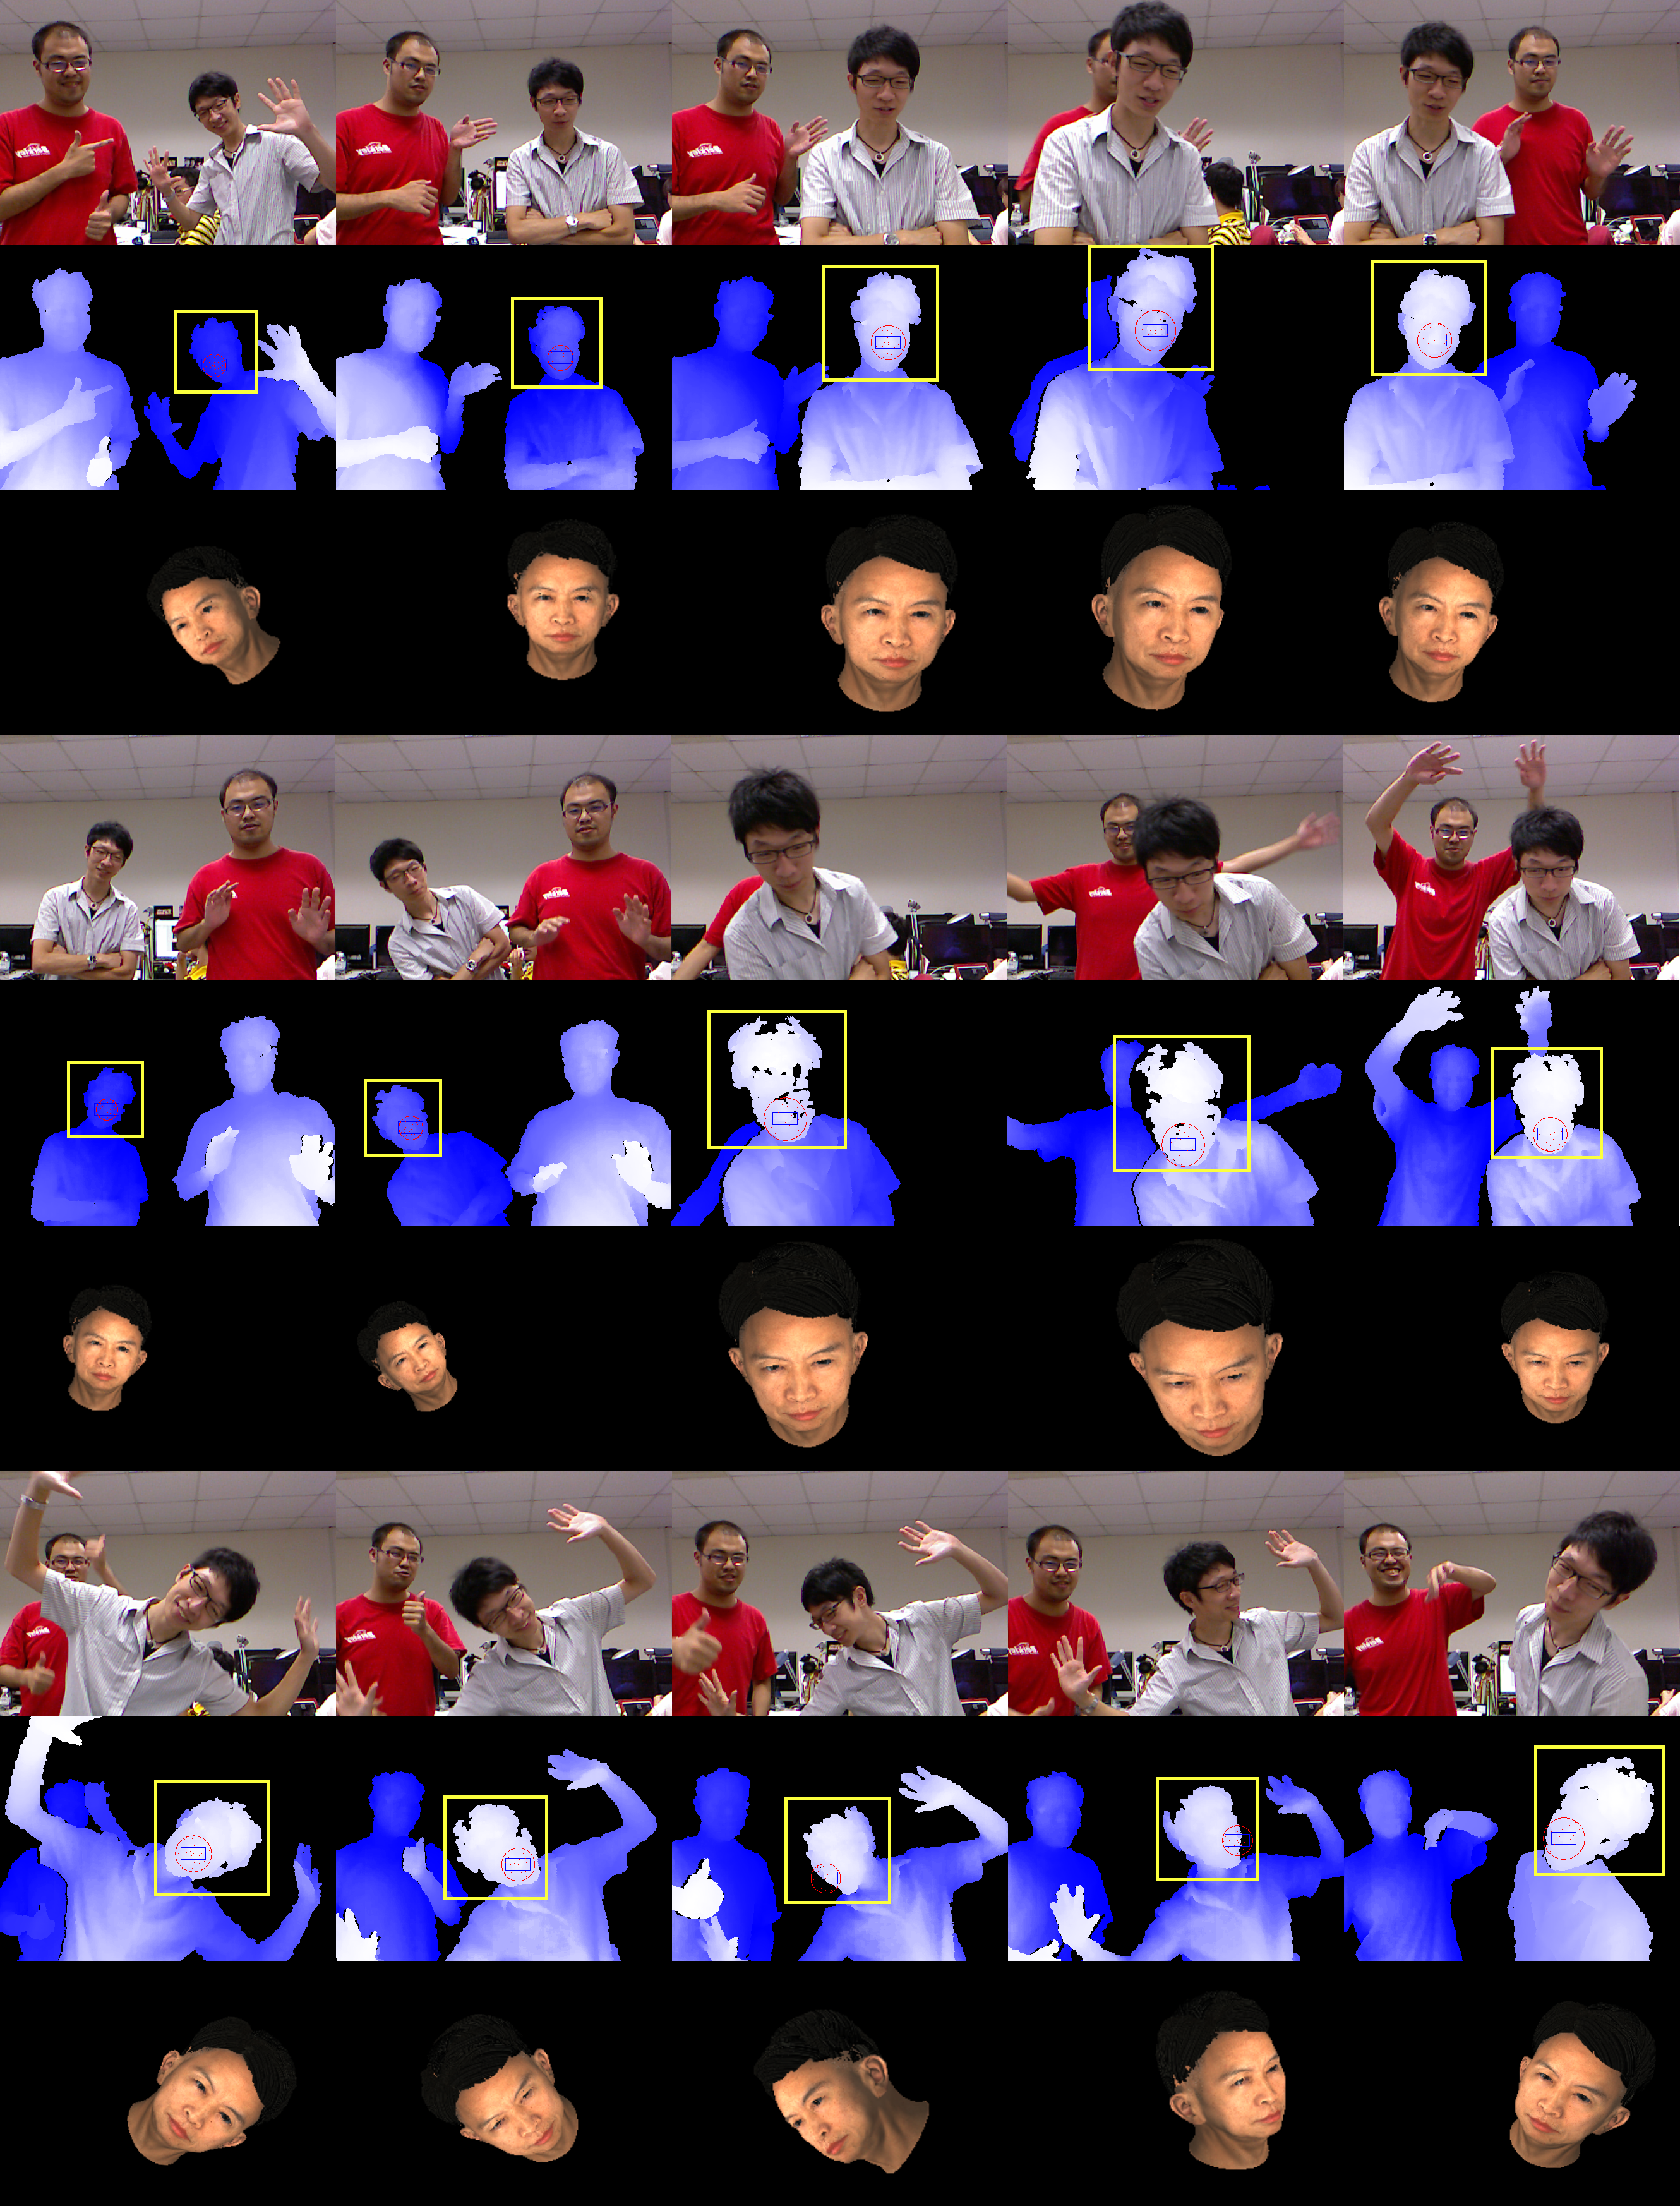
\includegraphics[width=1.0\linewidth]{./figure/Tantofish_Free_Result.png}
\caption{Experimental results of optimization solution. Tracking-based method successfully prevent the system from being affected by other user in the scene.}
\label{f:m2 result tantofish 3}       % Give a unique label
\end{figure}

\begin{figure}
\includegraphics[width=1.0\linewidth]{./figure/StreetDance.png}
\caption{Experimental results of optimization solution - Street dancing.}
\label{f:m2 result tantofish 4}       % Give a unique label
\end{figure}


Figure \ref{f:m2 result tantofish} shows some experimental results of optimization solution (method 2). The first column shows the poses that the user performs. The second column shows the corresponding depth map captured by Kinect. The third column shows the estimated poses. The fourth column overlaps the estimated poses with the observed depth map. Our experiment shows that this method succeeds in estimating the head pose within the range of $\pm 100^{\circ}$ yaw, $\pm 60^{\circ}$ pitch and $\pm 180^{\circ}$ roll rotations. It also shows that this method is more robust and precise than the least square method (method 1). 

Figure \ref{f:m2 result biwi 01} shows more results of the iterative optimization method. These results are estimated from one set of the BIWI database provided by ETH. 

\begin{figure}
\centering
\includegraphics[width=0.5\linewidth]{./figure/ResultCompare.pdf}
\caption{Accuracy of the system in terms of percentage of correctly estimated poses as a function of the angle error threshold using the BIWI database and is compared with \cite{fanelli_DAGM11}}
\label{f:m2 result tantofish 5}       % Give a unique label
\end{figure}


We implement our system on a PC with Intel Core 2 Due CPU P8600 (2.4 GHz), and both of the proposed methods can achieve 30 fps real-time responses.
\chapter{Conclusion and Future Work}
\label{c:conclusion}

\section{Conclusion}

\section{Future Work}


\backmatter

\addcontentsline{toc}{chapter}{\bibname}
% \bibliographystyle{abbrv}
\bibliographystyle{plain}
% input your reference here
\bibliography{reference}

\appendix

\includepdf[pages=1-2]{resume.pdf}
\end{document}
